\subsection{Precision Voltage Module (PV) }
\label{sec:PV}

The Precision Voltage Module (PV) provides a regulated \SI{2.5}{\volt} supply rail for SV and CO.


\subsubsection{Requirements}

The precision of PV has an impact on the upper threshold of CO. Given that the ambient temperature
varies between  \SI{0}{\degreeCelsius}  and  \SI{30}{\degreeCelsius} the temperature drift should be small.


\subsubsection{Implementation}


\begin{figure}[h]
    \centering
    \includegraphics[width=1.0\textwidth]{PO/PV/PV}
    % \caption{CO - schematic}
\end{figure}

\begin{table}[H]
    \centering
    \begin{threeparttable}[b]
        \begin{tabularx}{\linewidth}{ >
                    {\hsize=.25\hsize}X >
                    {\hsize=0.5\hsize}X >
                    {\hsize=.25\hsize}X  >
                    {\hsize=.5\hsize}X >
                    {\hsize=.25\hsize}X  >
                    {\hsize=3\hsize}X
            }
                  & \multicolumn{4}{c}{pin} &                                                              \\
            \cmidrule(lr){3-6}
            Id    & Net                     & Nb. & Name          & Type                 & Function        \\
            \midrule
            $U_1$ & \Gnd                    & 1   & \texttt{GND}  & \Gnd                 &                 \\
            $U_1$ & \Gnd                    & 2   & \texttt{GND}  & \Gnd                 &                 \\
            $U_1$ & EN                      & 3   & \texttt{EN}   & \leftharpoonup       & enable output   \\
            $U_1$ & .B                      & 4   & \texttt{VIN}  & \leftarrow           & input           \\
            $U_1$ & NR                      & 5   & \texttt{NR}   & \leftrightsquigarrow & noise reduction \\
            $U_1$ & .2V5                    & 6   & \texttt{VREF} & \rightarrow          & output          \\
            $C_1$ & .B                      & 1   & \texttt{1}    &                      &                 \\
            $C_1$ & \Gnd                    & 2   & \texttt{2}    & \Gnd                 &                 \\
            $C_2$ & .B                      & 1   & \texttt{1}    &                      &                 \\
            $C_2$ & \Gnd                    & 2   & \texttt{2}    & \Gnd                 &                 \\
            $C_3$ & NR                      & 1   & \texttt{1}    &                      &                 \\
            $C_3$ & \Gnd                    & 2   & \texttt{2}    & \Gnd                 &                 \\
            $C_4$ & .2V5                    & 1   & \texttt{1}    &                      &                 \\
            $C_4$ & \Gnd                    & 2   & \texttt{2}    & \Gnd                 &                 \\
            $C_5$ & .2V5                    & 1   & \texttt{1}    &                      &                 \\
            $C_5$ & \Gnd                    & 2   & \texttt{2}    & \Gnd                 &                 \\
        \end{tabularx}
    \end{threeparttable}
    %\caption{WD - Pin mapping}
\end{table}

\begin{table}[H]
    \centering
    \begin{threeparttable}[b]
        \begin{tabularx}{\linewidth}{
                >{\hsize=0.25\hsize}X
                >{\hsize=0.75\hsize}X
                >{\hsize=1.25\hsize}X
                >{\hsize=0.5\hsize}X
                >{\hsize=2.25\hsize}X}
            \toprule
            Id    & Desc                               & Order Code        & Package  & Rationale \\
            \midrule
            $U_1$ & \cite{ti_ref35_2022}               & REF35250QDBVR/921 & SOT-23-6 &           \\
            $C_1$ & \SI{1}{\micro\farad}, \SI{16}{\V}  & generic           & 0603     &           \\
            $C_2$ & \SI{100}{\nano\farad}, \SI{16}{\V} & generic           & 0603     &           \\
            $C_3$ & \SI{100}{\nano\farad}, \SI{16}{\V} & generic           & 0603     &           \\
            $C_4$ & \SI{1}{\micro\farad}, \SI{16}{\V}  & generic           & 1206     &           \\
            $C_5$ & \SI{10}{\nano\farad}, \SI{16}{\V}  & generic           & 0603     &           \\
            \bottomrule
        \end{tabularx}
    \end{threeparttable}
    \caption{PV - BOM}
    \label{table:wd1}
\end{table}

\begin{table}[H]
    \centering
    \begin{threeparttable}[b]
        \begin{tabularx}{\linewidth}{ >{\hsize=.15\hsize}X >{\hsize=1.35\hsize}X >{\hsize=1.5\hsize}X }
            \toprule
            Id & Issue                                                      & Potential solutions                        \\
            \midrule
            1  & The choice of 1.9V is not ideal, the threshold is too high & move the compairison function to the \mu C \\
            \bottomrule
        \end{tabularx}
    \end{threeparttable}
    \caption{CR - issues}
\end{table}
\clearpage